\documentclass[aspectratio=169]{beamer}

\usetheme{Madrid}
\usecolortheme{dolphin}
\usefonttheme{professionalfonts}

\usepackage[T1]{fontenc}
\usepackage[scaled=0.96]{helvet}
\usepackage{microtype}
\usepackage{graphicx}
\usepackage{booktabs}
\usepackage{xcolor}

\renewcommand{\familydefault}{\sfdefault}

\definecolor{PrimaryBlue}{HTML}{1F4E79}
\definecolor{PrimaryBlueDark}{HTML}{173B5C}
\definecolor{SecondaryTeal}{HTML}{2A7F78}
\definecolor{WarmAccent}{HTML}{C56B2C}
\definecolor{LightBlue}{HTML}{EAF2F8}
\definecolor{LightTeal}{HTML}{E8F4F2}
\definecolor{TextInk}{HTML}{1B2631}
\definecolor{MutedText}{HTML}{5D6D7E}

\setbeamercolor{palette primary}{fg=white,bg=PrimaryBlue}
\setbeamercolor{palette secondary}{fg=white,bg=SecondaryTeal}
\setbeamercolor{palette tertiary}{fg=white,bg=PrimaryBlueDark}
\setbeamercolor{palette quaternary}{fg=white,bg=WarmAccent}
\setbeamercolor{structure}{fg=PrimaryBlue}
\setbeamercolor{normal text}{fg=TextInk,bg=white}
\setbeamercolor{frametitle}{fg=white,bg=PrimaryBlue}
\setbeamercolor{title}{fg=white,bg=PrimaryBlue}
\setbeamercolor{subtitle}{fg=LightBlue,bg=PrimaryBlue}
\setbeamercolor{author}{fg=white,bg=PrimaryBlue}
\setbeamercolor{institute}{fg=LightBlue,bg=PrimaryBlue}
\setbeamercolor{date}{fg=LightBlue,bg=PrimaryBlue}
\setbeamercolor{block title}{fg=white,bg=PrimaryBlue}
\setbeamercolor{block body}{fg=TextInk,bg=LightBlue}
\setbeamercolor{block title example}{fg=white,bg=SecondaryTeal}
\setbeamercolor{block body example}{fg=TextInk,bg=LightTeal}
\setbeamercolor{block title alerted}{fg=white,bg=WarmAccent}
\setbeamercolor{block body alerted}{fg=TextInk,bg=WarmAccent!12}
\setbeamercolor{item}{fg=SecondaryTeal}
\setbeamercolor{subitem}{fg=PrimaryBlue}
\setbeamercolor{section in toc}{fg=PrimaryBlue}
\setbeamercolor{subsection in toc}{fg=MutedText}
\setbeamercolor{footline}{fg=MutedText,bg=white}

\setbeamerfont{title}{size=\Huge,series=\bfseries}
\setbeamerfont{subtitle}{size=\large}
\setbeamerfont{frametitle}{size=\Large,series=\bfseries}
\setbeamerfont{block title}{series=\bfseries}
\setbeamerfont{footline}{size=\scriptsize}

\setbeamertemplate{navigation symbols}{}
\setbeamertemplate{blocks}[rounded][shadow=false]
\setbeamertemplate{itemize item}{\raise0.15ex\hbox{\scriptsize$\blacktriangleright$}}
\setbeamertemplate{itemize subitem}{\raise0.15ex\hbox{\tiny$\bullet$}}
\setbeamertemplate{enumerate item}{\insertenumlabel.}
\setbeamertemplate{section in toc}[sections numbered]
\setbeamertemplate{footline}{
  \hfill
  \usebeamerfont{footline}\usebeamercolor[fg]{footline}
  \insertframenumber/\inserttotalframenumber\hspace{0.45cm}\vspace{0.25cm}
}

\setbeamersize{text margin left=0.8cm,text margin right=0.8cm}
\linespread{1.04}

\titlegraphic{}

\usepackage{tikz}
\usetikzlibrary{arrows.meta,calc}

\title{Migrating Search}
\subtitle{From PostgreSQL \texttt{(pg\_trgm)} to Elasticsearch \texttt{(BM25)}}
\author{Amir Hossein Rassafi}
\institute{Head of Platform at Condukt\\amir-h-rassafi.github.io}
\date{May 2026}

\begin{document}

% Slide title rule: content slide titles must use the story section as the main piece,
% followed by a short 1-5 word current-slide label: Section: Slide Label.
% Keep the longer explanatory wording only on The Story agenda slide.

\begin{frame}[plain]
  \vspace*{0.25cm}
  \begin{columns}[T,totalwidth=\textwidth]
    \column{0.5\textwidth}
      
\includegraphics[height=0.58cm]{assets/logos/condukt-logo-black.png}
    \column{0.5\textwidth}
      \raggedleft
\includegraphics[height=0.62cm]{assets/logos/elasticsearch.png}
  \end{columns}

  \vfill

  \begin{beamercolorbox}[wd=\textwidth,sep=0.48cm,center,rounded=true]{title}
    {\Huge\bfseries\inserttitle\par}
    \vspace{0.18cm}
    {\large\insertsubtitle\par}
  \end{beamercolorbox}

  \vspace{0.78cm}
  \begin{center}
    {\Large\bfseries\textcolor{PrimaryBlue}{\insertauthor}\par}
    \vspace{0.14cm}
    {\normalsize\bfseries\textcolor{SecondaryTeal}{Head of Platform at Condukt}\par}
    \vspace{0.08cm}
    {\small\textcolor{MutedText}{amir-h-rassafi.github.io}\par}
  \end{center}

  \vfill

  \begin{center}
    {\small\textcolor{MutedText}{\insertdate}}
  \end{center}
\end{frame}

\begin{frame}{The Story}
  \vspace{0.2cm}
  \begin{enumerate}
    \item \hyperlink{sec:problem}{\textbf{Problem \& Goal}}\\[-0.02cm]
      \hyperlink{sec:problem}{{\small\textcolor{MutedText}{Why and how this became an initiative}}}
    \item \hyperlink{sec:search-concepts}{\textbf{Search Concepts}}\\[-0.02cm]
      \hyperlink{sec:search-concepts}{{\small\textcolor{MutedText}{Text similarity vs search}}}
    \item \hyperlink{sec:migration-design}{\textbf{Migration Design}}\\[-0.02cm]
      \hyperlink{sec:migration-design}{{\small\textcolor{MutedText}{Moving data without overloading PostgreSQL}}}
    \item \hyperlink{sec:index-design}{\textbf{Index Design}}\\[-0.02cm]
      \hyperlink{sec:index-design}{{\small\textcolor{MutedText}{Recreating fuzzy-name signals in Elasticsearch}}}
    \item \hyperlink{sec:validation}{\textbf{Validation}}\\[-0.02cm]
      \hyperlink{sec:validation}{{\small\textcolor{MutedText}{Proving relevance before production rollout}}}
    \item \hyperlink{sec:outcome}{\textbf{Outcome}}\\[-0.02cm]
      \hyperlink{sec:outcome}{{\small\textcolor{MutedText}{Latency gains, trade-offs, and lessons}}}
  \end{enumerate}
\end{frame}

\section*{Scope}

\begin{frame}{Scope: Boundaries}
  \footnotesize
  \begin{columns}[T,totalwidth=\textwidth]
    \column{0.48\textwidth}
      \begin{block}{What this story covers}
        \begin{itemize}
          \item PostgreSQL \texttt{pg\_trgm} to Elasticsearch BM25.
          \item CDC-backed data movement and indexer shape.
          \item Ranking validation and production trade-offs.
        \end{itemize}
      \end{block}

    \column{0.48\textwidth}
      \begin{alertblock}{What this is not}
        \begin{itemize}
          \item Vector search or embeddings.
          \item RAG context matching or answer generation.
          \item Replacing expert judgement with metrics.
        \end{itemize}
      \end{alertblock}
  \end{columns}

  \vspace{0.18cm}
  {\scriptsize\textcolor{MutedText}{The same foundations still matter for RAG and hybrid search: freshness, identity, ranking, and observability.}}
\end{frame}


\section{Problem \& Goal}
\subsection{Why and how this became an initiative}

\begin{frame}{Problem \& Goal: Initiative}
  \hypertarget{sec:problem}{}
  \begin{itemize}
    \item The search covers multilingual company and legal-entity names, with spelling and spacing variations.
    \item The current search worked and users \textbf{trusted} its \textbf{fuzzy matching} behavior.
    \item It ran on PostgreSQL with \textbf{16 CPU} cores and \textbf{64 GB} memory.
    \item At around \textbf{10M} records, \textbf{p99} latency was about \textbf{10 seconds}.
    \item Maximum sustainable \textbf{throughput} was around \textbf{2 requests per second}.
  \end{itemize}

  \vspace{0.5cm}
  \begin{block}{Goal}
    Bring \textbf{p99} search latency \textbf{under 1 second}, increase \textbf{throughput} by at least \textbf{10x}, and \textbf{preserve the ranking behavior} users already trusted.
  \end{block}
\end{frame}

\begin{frame}{Problem \& Goal: Options}
  After applying the available PostgreSQL and index optimizations, the remaining options were:
  \begin{columns}[T,totalwidth=\textwidth]
    \column{0.48\textwidth}
      \begin{itemize}
        \item Scale up the database.
          \begin{itemize}
            \item More CPU helped throughput and concurrency, but not single-query latency.
            \item It also kept search coupled to an expensive source-of-truth database.
          \end{itemize}
        \item Move search to a dedicated system.
      \end{itemize}

    \column{0.48\textwidth}
      \begin{block}{}
        \small
        \begin{tabular}{@{}ll@{}}
          Current p99 & \textcolor{WarmAccent}{\rule{3.2cm}{0.18cm}} 10s \\
          Target p99 & \textcolor{SecondaryTeal}{\rule{0.35cm}{0.18cm}} <1s \\
          Current RPS & \textcolor{WarmAccent}{\rule{0.45cm}{0.18cm}} 2 \\
          Target RPS & \textcolor{SecondaryTeal}{\rule{3.8cm}{0.18cm}} $\geq$20
        \end{tabular}
      \end{block}
  \end{columns}
\end{frame}

\begin{frame}{Problem \& Goal: Tool Investigation}
  Shortlist: Typesense, Meilisearch, and Elasticsearch.
  \vspace{0.2cm}
  \begin{itemize}
    \item Scale: partition the index and grow beyond one node.
    \item Availability: replicas and established cluster operations.
    \item Search control: tune analyzers, fields, and ranking signals.
  \end{itemize}
  \begin{block}{Decision}
    Elasticsearch fit the search requirements and operating model. The latency target was an acceptance criterion; this slide is a requirements comparison, not a three-engine benchmark.
  \end{block}
\end{frame}

\section{Search Concepts}
\subsection{Text similarity vs search}

\begin{frame}{Search Concepts: Why This Matters}
  \hypertarget{sec:search-concepts}{}
  Because PostgreSQL \texttt{pg\_trgm} and Elasticsearch BM25 match and rank text differently, we need a few concepts before discussing the migration.

  \vspace{0.25cm}
  \begin{itemize}
    \item Trigram similarity: how the old search matched fuzzy text.
    \item Trigram indexes: why p99 latency still had a tail cost.
    \item BM25: how Elasticsearch scores analyzed search terms.
    \item Matching tradeoffs and query fuzziness: where behavior changes.
  \end{itemize}
\end{frame}

\begin{frame}{Search Concepts: Trigram Similarity}
  \begin{block}{What it is}
    A trigram is a rolling 3-character window. Similar strings share many windows, even when spelling or spacing differs.
  \end{block}

  \begin{columns}[T,totalwidth=\textwidth]
    \column{0.48\textwidth}
      \begin{itemize}
        \item Useful for typos, spacing differences, and fuzzy names.
        \item Character overlap needs no language-specific stemmer.
        \item Normalization still matters for accents, case, and punctuation.
      \end{itemize}

    \column{0.44\textwidth}
      \begin{block}{Why it fits}
        \centering
        \large Names are short, noisy, and\\[0.12cm]
        users usually know only an approximate spelling.
      \end{block}
  \end{columns}
\end{frame}

\begin{frame}{Search Concepts: Trigram Similarity Example}
  \begin{exampleblock}{PostgreSQL pads each word with spaces}
    \texttt{search} $\rightarrow$ \texttt{\{\_\_s, \_se, sea, ear, arc, rch, ch\_\}}\\[0.2cm]
    \texttt{serch} $\rightarrow$ \texttt{\{\_\_s, \_se, ser, erc, rch, ch\_\}}
  \end{exampleblock}
  \small \texttt{\_} represents a space; every fragment has three characters.
  \vspace{0.3cm}
  \begin{block}{Four shared fragments, nine distinct fragments}
    \centering \Large similarity = 4 / 9 $\approx$ 0.44
  \end{block}
\end{frame}

\begin{frame}{Search Concepts: Trigram Indexes}
  \begin{itemize}
    \item Common fragments can produce many candidate names.
    \item Lower similarity thresholds trade more work for more recall.
    \item Returning 20 results can still require ranking many candidates.
  \end{itemize}
  \begin{block}{Query plan matters}
    GIN filtering plus similarity sorting and GiST nearest-neighbor search have different costs. These latency results describe our workload, not a universal PostgreSQL limit.
  \end{block}
\end{frame}

\begin{frame}[fragile]{Search Concepts: Trigram Queries}
  \begin{columns}[T,totalwidth=\textwidth]
    \column{0.48\textwidth}
      \begin{block}{PostgreSQL: similarity}
        \scriptsize
\begin{verbatim}
SELECT name,
       similarity(name, 'serch')
FROM companies
WHERE name % 'serch'
ORDER BY
  similarity(name, 'serch') DESC
LIMIT 20;
\end{verbatim}
      \end{block}
    \column{0.48\textwidth}
      \begin{block}{Elasticsearch: analyzed terms}
        \scriptsize
\begin{verbatim}
GET companies/_search
{
  "size": 20,
  "query": {
    "match": {
      "name.ngram": "serch"
    }
  }
}
\end{verbatim}
      \end{block}
  \end{columns}
  \vspace{0.15cm}
  \small The Elasticsearch example analyzes both names and queries into trigrams. BM25 scores their shared terms; it does not reproduce PostgreSQL's similarity formula.
\end{frame}
\begin{frame}{Search Concepts: BM25 Formula}
  \begin{columns}[T,totalwidth=\textwidth]
    \column{0.44\textwidth}
      \begin{block}{Analyzer creates terms}
        \texttt{apple apple banana}\\[0.2cm]
        $\rightarrow$ \texttt{apple}, \texttt{apple}, \texttt{banana}
      \end{block}

      \begin{block}{Base idea}
        \centering
        $\text{score} \approx tf \times idf$
      \end{block}

      \begin{itemize}
        \item $tf$: term frequency in this document.
        \item $idf$: rarity across all documents.
      \end{itemize}

    \column{0.52\textwidth}
      \begin{block}{BM25 extension}
        \scriptsize
        \[
          \sum_{t \in q} \operatorname{idf}(t) \cdot
          \frac{tf(t,d)(k_1 + 1)}
          {tf(t,d) + k_1\left(1 - b + b\frac{|d|}{avgdl}\right)}
        \]
      \end{block}

      \begin{itemize}
        \item Rare terms still matter most.
        \item Repeated terms help, but the gain saturates.
        \item Long noisy documents are normalized against average length.
      \end{itemize}
  \end{columns}

  \vspace{0.05cm}
  \begin{block}{Key distinction}
    \texttt{pg\_trgm} is text similarity. BM25 scores analyzed search terms.
  \end{block}
\end{frame}

\begin{frame}{Search Concepts: Matching Tradeoffs}
  \begin{columns}[T,totalwidth=\textwidth]
    \column{0.48\textwidth}
      \begin{block}{Similarity wins}
        Query: \texttt{jon smyth}\\[0.15cm]
        Record: \texttt{john smith}
      \end{block}


    \column{0.48\textwidth}
      \begin{block}{BM25 wins}
        Query: \texttt{senior backend engineer}\\[0.15cm]
        Record: \texttt{backend engineer with search experience}
        \\[0.15cm]{\scriptsize With simple word / space tokenization}
      \end{block}

  \end{columns}
\end{frame}

\begin{frame}{Search Concepts: Matching Tradeoffs: What Changes}
  \begin{columns}[T,totalwidth=\textwidth]
    \column{0.48\textwidth}
      \begin{itemize}
        \item Same name intent, different spelling.
        \item Shared character fragments keep the match close.
        \item BM25 may miss or weaken it because exact terms differ.
      \end{itemize}
    \column{0.48\textwidth}
      \begin{itemize}
        \item Space-separated terms contribute to relevance.
        \item Rare terms carry more signal than common ones.
        \item Similarity alone treats this as broad text overlap.
      \end{itemize}
  \end{columns}
\end{frame}

\begin{frame}{Search Concepts: Query Fuzziness}
  \scriptsize
  \begin{columns}[T,totalwidth=\textwidth]
    \column{0.48\textwidth}
      \begin{block}{Query shape}
        \texttt{match} analyzes text into terms and BM25 scores the matching documents.
      \end{block}

      \begin{itemize}
        \item Filters restrict matches without adding to the score.
        \item Text clauses score the remaining candidates.
        \item Boosts decide which fields matter more.
      \end{itemize}


    \column{0.48\textwidth}
      \begin{block}{Fuzziness}
        \texttt{fuzziness: AUTO} expands terms to nearby spellings.
      \end{block}

      \begin{itemize}
        \item Better recall for typos and name variants.
        \item More expansions increase query work.
        \item Prefix length and max expansions limit the cost.
      \end{itemize}

  \end{columns}

  \vspace{0.05cm}
  \begin{block}{Latency tradeoff}
    Target fuzziness where needed: broad matching can raise p99.
  \end{block}
\end{frame}




\begin{frame}{Search Concepts: Query Shape}
  \begin{block}{Our query combines six \texttt{should} clauses}
    Exact name, prefix, fuzzy prefix, fuzzy text, whitespace-tokenized text, and word shingles.
  \end{block}
  \begin{itemize}
    \item \texttt{minimum\_should\_match: 1} requires one matching clause.
    \item Matching clauses contribute to the combined score.
    \item Boosts weight signals; they do not guarantee a fixed ranking order.
  \end{itemize}
  \small The complete query and its boosts follow in Index Design.
\end{frame}

\begin{frame}[fragile]{Search Concepts: Typo Example}
  \begin{columns}[T,totalwidth=\textwidth]
    \column{0.56\textwidth}
      \small
\begin{verbatim}
{
  "match": {
    "name": {
      "query": "progema fastighetts",
      "boost": 70,
      "fuzziness": "auto"
    }
  }
}
\end{verbatim}
    \column{0.40\textwidth}
      \begin{exampleblock}{Example candidate}
        Progema Fastighets AB
      \end{exampleblock}
      \small \texttt{fastighetts} differs from \texttt{fastighets} by one insertion.
      \vspace{0.2cm}

      This is the fuzzy name clause from our query. A separate prefix clause uses \texttt{fuzziness: "1"}.
  \end{columns}
\end{frame}

\section{Migration Design}
\subsection{Moving data without overloading PostgreSQL}

\begin{frame}{Migration Design: Requirements}
  \hypertarget{sec:migration-design}{}
  \begin{itemize}
    \item Deploy Elasticsearch quickly with low operational overhead.
    \item Replicate required PostgreSQL data into Elasticsearch.
    \item Preserve fuzzy, language-agnostic name search behavior.
    \item Benchmark old and new ranking behavior.
    \item Prove the new path before production rollout.
  \end{itemize}
\end{frame}

\begin{frame}{Migration Design: Before And After}
  \begin{block}{Before}
    Application $\rightarrow$ PostgreSQL\\[0.15cm]
    Transactional reads/writes and \texttt{pg\_trgm} search share the database.
  \end{block}
  \vspace{0.15cm}
  \begin{block}{After}
    Application $\rightarrow$ PostgreSQL for transactional data\\[0.15cm]
    Application $\rightarrow$ Elasticsearch for search\\[0.15cm]
    PostgreSQL $\rightarrow$ CDC pipeline $\rightarrow$ Elasticsearch
  \end{block}
  \small The migration changes search queries and adds asynchronous indexing.
\end{frame}

\begin{frame}{Migration Design: Data Path}
  \centering
  \vfill
  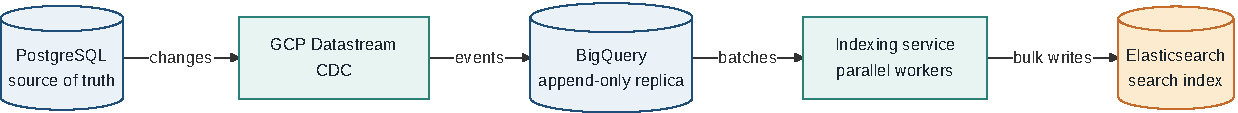
\includegraphics[width=0.98\textwidth]{diagrams/02-target-architecture-cropped.pdf}
  \vspace{0.3cm}

  \small PostgreSQL owns the data; BigQuery holds change history; Elasticsearch serves search.
  \vfill
\end{frame}

\begin{frame}{Migration Design: Elasticsearch Cluster}
  \begin{itemize}
    \item 3 data nodes, each with 4 cores and 8 GB RAM.
    \item 3 primary shards; 1 replica per primary (6 shard copies).
    \item Elasticsearch handles allocation and request routing.
    \item Writes go through primaries and replicate to in-sync copies.
    \item Reads can use primary or replica copies.
  \end{itemize}
  \begin{block}{Two independent kinds of partitioning}
    Elasticsearch shards distribute the index. Indexer partitions distribute CDC processing; their counts need not match.
  \end{block}
\end{frame}

\begin{frame}{Migration Design: Document Identity}
  \begin{itemize}
    \item Reuse the PostgreSQL row ID as the Elasticsearch document ID.
    \item Trace the same entity across the database, CDC, and search.
    \item Repeating a document replacement avoids duplicate documents.
  \end{itemize}
  \begin{block}{Replay also needs ordering}
    A stable ID alone cannot stop an older change overwriting a newer one. Preserve source order or enforce source versions, including deletes.
  \end{block}
\end{frame}

\begin{frame}{Migration Design: Indexer Partitions}
  \centering
  \begin{block}{Deterministic assignment}
    \centering \texttt{partition = hash(entity\_unique\_id) \% N}
  \end{block}
  \vspace{0.2cm}
  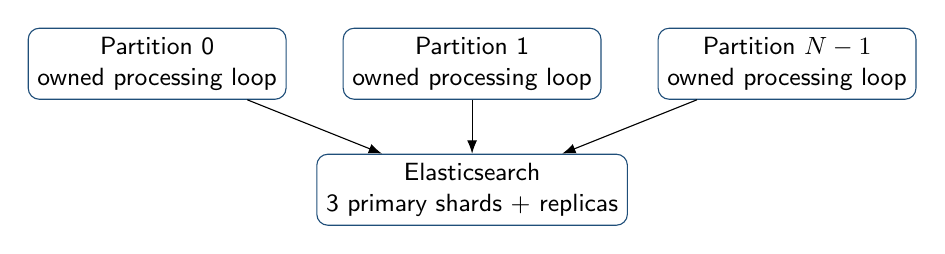
\begin{tikzpicture}[every node/.style={draw=PrimaryBlue,rounded corners,align=center,font=\small,minimum height=0.8cm},>=Latex]
    \node (a) at (0,0) {Partition 0\\owned processing loop};
    \node (b) at (4,0) {Partition 1\\owned processing loop};
    \node (c) at (8,0) {Partition $N-1$\\owned processing loop};
    \node (es) at (4,-1.6) {Elasticsearch\\3 primary shards + replicas};
    \draw[->] (a) -- (es);
    \draw[->] (b) -- (es);
    \draw[->] (c) -- (es);
  \end{tikzpicture}
  \vspace{0.15cm}

  \small One active owner per partition; a worker process can host multiple loops.\\
  $N$ describes indexer partitions, not Elasticsearch shards.
\end{frame}

\begin{frame}{Migration Design: Timestamp Lag}
  \centering
  \vspace{-0.05cm}
  \resizebox{0.84\textwidth}{!}{\begingroup
\tikzset{
  system box/.style={
    draw=TextInk,
    line width=0.6pt,
    rounded corners=3pt,
    fill=white,
    align=center,
    font=\tiny,
    minimum width=1.25cm,
    minimum height=0.48cm
  },
  indexer box/.style={
    system box,
    fill=SecondaryTeal!10
  },
  flow arrow/.style={
    -{Latex[length=1.5mm,width=1.1mm]},
    line width=0.45pt,
    draw=TextInk
  },
  timeline arrow/.style={
    -{Latex[length=2.2mm,width=1.6mm]},
    line width=0.65pt,
    draw=TextInk
  },
  marker line/.style={
    dashed,
    line width=0.45pt,
    draw=TextInk
  },
  note text/.style={
    align=center,
    font=\tiny,
    text=TextInk
  },
  tiny note/.style={
    align=center,
    font=\tiny,
    text=TextInk
  },
  phase label/.style={
    align=center,
    font=\scriptsize,
    text=TextInk
  }
}

\begin{tikzpicture}[
  x=1cm,
  y=1cm,
  line cap=round,
  line join=round,
  font=\sffamily
]
  \definecolor{GuardGreen}{HTML}{1E9C3F}
  \definecolor{RiskRed}{HTML}{C92A2A}

  \node[system box] (pg) at (1.00,4.30) {PostgreSQL};
  \node[system box] (ds) at (3.15,4.30) {Datastream};
  \node[system box] (bq) at (5.20,4.30) {BigQuery};
  \node[indexer box] (idx) at (7.10,4.30) {Indexer};
  \node[system box, minimum width=1.45cm] (es) at (9.45,4.30) {Elasticsearch};

  \draw[flow arrow] (pg.east) -- (ds.west);
  \draw[flow arrow] (ds.east) -- (bq.west);
  \draw[flow arrow] (bq.east) -- (idx.west);
  \draw[flow arrow] (idx.east) -- (es.west);

  \coordinate (t0) at (0.75,2.06);
  \coordinate (t1) at (11.25,2.06);
  \draw[timeline arrow] (t0) -- (t1);
  \node[note text, anchor=west] at (11.34,1.97) {now};

  \foreach \x in {1.00,3.15,5.20,7.10} {
    \draw[TextInk,line width=0.55pt] (\x,1.91) -- (\x,2.21);
  }
  \coordinate (bqVisible) at (5.20,2.48);
  \coordinate (readPoint) at (7.38,2.06);
  \coordinate (bufferStart) at (7.62,2.06);
  \coordinate (bufferEnd) at (8.84,2.06);
  \coordinate (unsafeStart) at (9.04,2.06);
  \coordinate (unsafeEnd) at (10.25,2.06);

  \draw[marker line] (bq.south) -- (bqVisible) -- (5.20,2.28);
  \draw[marker line] (idx.south) -- (readPoint);

  \draw[fill=GuardGreen!30,draw=GuardGreen,line width=0.75pt] (readPoint) circle (0.11);
  \node[tiny note, text=GuardGreen, anchor=south] at (7.38,2.34) {safe read cutoff};

  \draw[draw=MutedText,line width=0.45pt] (bufferStart) -- (bufferEnd);
  \foreach \x in {7.66,7.82,...,8.66} {
    \draw[MutedText!55,line width=0.3pt] (\x,1.90) -- ++(0.22,0.32);
  }
  \node[tiny note] at (8.23,1.55) {lag buffer\\few minutes};

  \draw[fill=RiskRed!12,draw=RiskRed,line width=0.7pt] (9.04,1.88) rectangle (10.25,2.24);
  \foreach \x in {9.10,9.26,...,10.02} {
    \draw[RiskRed!62,line width=0.3pt] (\x,1.89) -- ++(0.22,0.32);
  }
  \node[tiny note, text=RiskRed] at (9.64,2.72) {do not read newest\\CDC window};
  \draw[RiskRed,line width=0.5pt] (9.64,2.48) -- (9.64,2.26);

  \node[phase label] at (4.05,1.35) {already indexed};
  \node[note text] at (6.05,0.70) {Guardrail: lag keeps checkpoint from passing CDC rows that have not arrived yet.};
\end{tikzpicture}
\endgroup
}
\end{frame}

\begin{frame}{Migration Design: Checkpointing}
  \begin{block}{One partition's ordered batch}
    Read checkpoint $\rightarrow$ fetch rows $\rightarrow$ bulk write\\[0.2cm]
    Check every item $\rightarrow$ commit the partition checkpoint
  \end{block}
  \begin{itemize}
    \item Cursor: source timestamp, source sequence / LSN, document ID.
    \item Advance only past successfully handled events.
    \item On failure, retry from the last committed checkpoint.
  \end{itemize}
  \small An HTTP success response does not mean every bulk item succeeded.
\end{frame}

\begin{frame}{Migration Design: Partition State Machine}
  \centering
  \vspace{-0.05cm}
  \resizebox{0.92\textwidth}{!}{\begingroup
\tikzset{
  state box/.style={
    draw=TextInk,
    line width=0.55pt,
    rounded corners=3pt,
    fill=white,
    align=center,
    font=\tiny,
    minimum width=1.55cm,
    minimum height=0.58cm,
    inner xsep=4pt,
    inner ysep=3pt
  },
  active state/.style={
    state box,
    fill=LightBlue
  },
  shard box/.style={
    state box,
    fill=SecondaryTeal!10,
    minimum width=1.38cm,
    minimum height=0.66cm
  },
  invariant box/.style={
    draw=PrimaryBlue!70,
    line width=0.5pt,
    rounded corners=3pt,
    fill=PrimaryBlue!4,
    align=center,
    font=\tiny,
    text width=7.20cm,
    inner sep=5pt
  },
  note/.style={
    font=\tiny,
    text=SecondaryTeal,
    align=center
  },
  muted note/.style={
    font=\tiny,
    text=MutedText,
    align=center
  },
  arrow/.style={
    -{Latex[length=1.45mm,width=1.0mm]},
    line width=0.45pt,
    draw=TextInk
  },
  feedback/.style={
    -{Latex[length=1.25mm,width=0.9mm]},
    line width=0.42pt,
    draw=MutedText,
    dashed,
    rounded corners=5pt
  },
  guide/.style={
    line width=0.42pt,
    draw=TextInk
  }
}

\begin{tikzpicture}[
  x=1cm,
  y=1cm,
  line cap=round,
  line join=round,
  font=\sffamily
]
  \node[note] at (5.05,4.48) {One independent state machine per shard};

  \node[active state] (own) at (0.70,3.76) {Own\\shard $k$};
  \node[state box, minimum width=1.70cm] (read) at (2.72,3.76) {Read shard\\checkpoint};
  \node[state box, minimum width=1.78cm] (fetch) at (4.95,3.76) {Fetch ordered\\rows};
  \node[state box, minimum width=1.82cm] (write) at (7.18,3.76) {Bulk write\\(throttled)};
  \node[active state, minimum width=1.78cm] (commit) at (9.35,3.76) {Commit shard\\checkpoint};

  \draw[arrow] (own.east) -- (read.west);
  \draw[arrow] (read.east) -- (fetch.west);
  \draw[arrow] (fetch.east) -- (write.west);
  \draw[arrow] (write.east) -- (commit.west);
  \draw[feedback] (commit.south) -- ++(0,-0.48) -- ++(-8.65,0) -- (own.south);
  \node[muted note] at (5.05,2.98) {retry or next batch};

  \node[note] at (5.05,2.42) {\texttt{shard = hash(entity\_unique\_id) \% N}};
  \draw[guide] (2.05,1.94) -- (8.05,1.94);

  \node[shard box] (s0) at (2.05,1.28) {Shard 0\\unique IDs};
  \node[shard box] (s1) at (4.05,1.28) {Shard 1\\unique IDs};
  \node[muted note] at (5.55,1.31) {$\cdots$};
  \node[shard box] (sn) at (7.25,1.28) {Shard $N-1$\\unique IDs};

  \draw[arrow] (2.05,1.94) -- (s0.north);
  \draw[arrow] (4.05,1.94) -- (s1.north);
  \draw[arrow] (7.25,1.94) -- (sn.north);

  \node[invariant box] at (5.05,0.18) {
    Sharding helps because workers do not fight for the same entity.\\
    One entity ID maps to one shard, one worker path, and one checkpoint stream.
  };
\end{tikzpicture}
\endgroup
}
\end{frame}

\section{Index Design}
\subsection{Recreating fuzzy-name signals in Elasticsearch}

\begin{frame}[fragile]{Index Design: Elasticsearch Multi-fields}
  \hypertarget{sec:index-design}{}
  \scriptsize
\begin{verbatim}
"name": {
  "type": "text", "analyzer": "name_words",
  "fields": {
    "normalized_keyword": {
      "type": "keyword", "normalizer": "name_exact"
    },
    "prefix": {
      "type": "text", "analyzer": "name_prefix",
      "search_analyzer": "name_words"
    },
    "whitespace_tokenizer": {
      "type": "text", "analyzer": "name_whitespace"
    },
    "word_shingle": {
      "type": "text", "analyzer": "name_shingle"
    }
  }
}
\end{verbatim}
  \small Actual query field names; analyzer definitions here remain illustrative.
\end{frame}

\begin{frame}{Index Design: Analyzer Choices}
  \begin{itemize}
    \item Normalize case consistently across indexed names and queries.
    \item Prefix field: index edge n-grams; search with whole word tokens.
    \item Whitespace field: split on spaces to retain a different token boundary signal.
    \item Shingle field: index and query adjacent word sequences.
  \end{itemize}
  \begin{block}{Test the tokens}
    Use \texttt{\_analyze} with short names, accents, abbreviations, and punctuation such as \texttt{A-TE}. A field name alone does not define its analyzer.
  \end{block}
\end{frame}

\begin{frame}{Index Design: Prefix Matching}
  \begin{exampleblock}{Input}
    \texttt{progema}
  \end{exampleblock}

  \vspace{0.05cm}
  \begin{center}
    \texttt{pr}, \texttt{pro}, \texttt{prog}, \texttt{proge}, \texttt{progem}, \texttt{progema}
  \end{center}

  \vspace{0.45cm}
  \begin{block}{Use case}
    Users often type only the beginning of a name and expect autocomplete-like behavior.
  \end{block}
\end{frame}

\begin{frame}{Index Design: Why Separate Prefixes}
  \begin{itemize}
    \item A dedicated prefix field exposes its gram lengths and analyzer.
    \item Its query clause can be weighted separately from exact matches.
    \item It fits the same multi-field design as our other name signals.
  \end{itemize}
  \begin{block}{Alternative: \texttt{search\_as\_you\_type}}
    Elasticsearch also provides built-in prefix and shingle subfields with configurable analysis. Long names or punctuation alone do not rule it out.
  \end{block}
  \small Choose based on required matching behavior and measured relevance/cost.
\end{frame}

\begin{frame}{Index Design: Character N-Grams}
  \begin{exampleblock}{Input}
    \texttt{progema}
  \end{exampleblock}

  \vspace{0.05cm}
  \begin{center}
    \texttt{pro}, \texttt{rog}, \texttt{oge}, \texttt{gem}, \texttt{ema}
  \end{center}

  \vspace{0.45cm}
  \begin{block}{Use case}
    An illustrative character-overlap signal. Our supplied query uses fuzzy text and prefix clauses; it does not query a separate n-gram field.
  \end{block}
\end{frame}

\begin{frame}{Index Design: Word Shingles}
  \begin{exampleblock}{Input: \texttt{progema fastighets ab}}
    Two-word shingles:\\[0.15cm]
    \texttt{progema fastighets}, \texttt{fastighets ab}\\[0.2cm]
    Three-word shingle:\\[0.15cm]
    \texttt{progema fastighets ab}
  \end{exampleblock}
  \begin{itemize}
    \item Shingles join adjacent tokens in their original order.
    \item They add phrase signals alongside individual words.
    \item They are a text-analysis technique, unrelated to \texttt{pgvector}.
  \end{itemize}
\end{frame}

\begin{frame}{Index Design: Size And Query Cost}
  \begin{center}
    \begin{tabular}{ll}
      \toprule
      Indexed form & Additional work \\
      \midrule
      Exact keyword & One normalized term per name \\
      Prefix & Several prefixes per word \\
      Whitespace text & Another token stream \\
      Word shingle & Additional adjacent-word terms \\
      \bottomrule
    \end{tabular}
  \end{center}
  \begin{block}{Measure the trade-off}
    Index a representative sample. Compare disk usage, indexing throughput, query latency, and relevance before retaining an extra field.
  \end{block}
\end{frame}

\begin{frame}[fragile]{Index Design: Our Search Query}
  \scriptsize
\begin{verbatim}
body = {"query": {"bool": {
    "should": [
        {"term": {"name.normalized_keyword":
            {"value": query, "boost": 300}}},
        {"match": {"name.prefix":
            {"query": query, "boost": 40}}},
        {"match": {"name.prefix":
            {"query": query, "boost": 40, "fuzziness": "1"}}},
        {"match": {"name":
            {"query": query, "boost": 70, "fuzziness": "auto"}}},
        {"match": {"name.whitespace_tokenizer":
            {"query": query, "boost": 30}}},
        {"match": {"name.word_shingle":
            {"query": query, "boost": 10}}},
    ],
    "minimum_should_match": 1,
}}}
\end{verbatim}
  \small Python request body; \texttt{query} is the same input string in every clause.
\end{frame}

\begin{frame}{Index Design: Query Weights}
  \small
  \begin{center}
    \begin{tabular}{lll}
      \toprule
      Field & Match behavior & Boost \\
      \midrule
      \texttt{name.normalized\_keyword} & Exact term & 300 \\
      \texttt{name.prefix} & Analyzed prefix & 40 \\
      \texttt{name.prefix} & Fuzziness 1 & 40 \\
      \texttt{name} & Fuzziness auto & 70 \\
      \texttt{name.whitespace\_tokenizer} & Analyzed text & 30 \\
      \texttt{name.word\_shingle} & Adjacent-word signal & 10 \\
      \bottomrule
    \end{tabular}
  \end{center}
  \begin{block}{How the signals combine}
    At least one clause must match. Scores add across matching clauses; both prefix clauses can contribute to the same result.
  \end{block}
\end{frame}

\section{Validation}
\subsection{Proving relevance before production rollout}

\begin{frame}{Validation: What MRR Measures}
  \hypertarget{sec:validation}{}
  Mean Reciprocal Rank: average $1 / \text{rank}$ of the first relevant result.
  \vspace{0.2cm}
  \begin{center}
    \begin{tabular}{lll}
      \toprule
      Query & First relevant result & Reciprocal rank \\
      \midrule
      A & Rank 1 & 1 \\
      B & Rank 2 & 0.5 \\
      C & Missing from top 20 & 0 \\
      \bottomrule
    \end{tabular}
  \end{center}
  \begin{block}{Illustrative MRR@20}
    $(1 + 0.5 + 0) / 3 = 0.50$\\[0.1cm]
    Higher is better; use the same queries, relevance labels, and cutoff.
  \end{block}
\end{frame}

\begin{frame}{Validation: Backtesting}
  \begin{itemize}
    \item Replay historical queries against both search systems.
    \item Use selected companies as candidate relevance labels.
    \item Inspect missing results and changes near the top.
    \item Supplement replay with generated cases and expert review.
  \end{itemize}
  \begin{block}{Reading the evidence}
    Historical selections can reflect the old ranking. MRR is useful for a paired evaluation; the result reported here is the separate human review.
  \end{block}
\end{frame}

\begin{frame}{Validation: Generated Cases}
  \begin{itemize}
    \item Generate realistic spelling-error cases.
    \item Include actual user typos and missing characters.
    \item Change spacing and casing.
    \item Remove words or groups of words.
    \item Test clean names and messy real-world inputs.
  \end{itemize}
\end{frame}

\begin{frame}{Validation: Human Judgement}
  \begin{columns}[T,totalwidth=\textwidth]
    \column{0.42\textwidth}
      \begin{itemize}
        \item Run the same query against both systems.
        \item Ask domain experts which result looked better.
        \item Treat \texttt{both} as acceptable ranking parity.
      \end{itemize}

      \vspace{0.25cm}
      \begin{block}{Decision signal}
        Elasticsearch was preferred or tied in 80\% of reviewed cases.
      \end{block}

    \column{0.54\textwidth}
      \centering
      \resizebox{0.95\linewidth}{!}{\begingroup
\tikzset{
  chart label/.style={
    font=\scriptsize,
    text=TextInk,
    align=left
  },
  pct label/.style={
    font=\tiny,
    text=MutedText,
    align=left
  },
  leader/.style={
    draw=MutedText,
    line width=0.45pt
  }
}

\begin{tikzpicture}[
  x=1cm,
  y=1cm,
  line cap=round,
  line join=round,
  font=\sffamily
]
  \definecolor{ChartBlue}{HTML}{4285F4}
  \definecolor{ChartRed}{HTML}{EA4335}
  \definecolor{ChartYellow}{HTML}{FBBC05}

  \coordinate (c) at (0,0);
  \def\r{1.45}

  \fill[ChartBlue] (c) -- (90:\r) arc[start angle=90,end angle=-92.16,radius=\r] -- cycle;
  \fill[ChartRed] (c) -- (-92.16:\r) arc[start angle=-92.16,end angle=-164.16,radius=\r] -- cycle;
  \fill[ChartYellow] (c) -- (-164.16:\r) arc[start angle=-164.16,end angle=-270,radius=\r] -- cycle;

  \draw[white,line width=0.45pt] (c) -- (90:\r);
  \draw[white,line width=0.45pt] (c) -- (-92.16:\r);
  \draw[white,line width=0.45pt] (c) -- (-164.16:\r);

  \fill[MutedText] (3:1.28) circle (0.025);
  \draw[leader] (3:1.28) -- (2.35,0.08);
  \node[chart label, anchor=west] at (2.38,0.15) {Elasticsearch};
  \node[pct label, anchor=west] at (2.38,-0.08) {50.6\%};

  \fill[MutedText] (156:1.24) circle (0.025);
  \draw[leader] (156:1.24) -- (-2.25,0.74);
  \node[chart label, anchor=east] at (-2.28,0.83) {Both};
  \node[pct label, anchor=east] at (-2.28,0.60) {29.4\%};

  \fill[MutedText] (235:1.12) circle (0.025);
  \draw[leader] (235:1.12) -- (-2.25,-1.05);
  \node[chart label, anchor=east] at (-2.28,-0.96) {PostgreSQL};
  \node[pct label, anchor=east] at (-2.28,-1.19) {20.0\%};
\end{tikzpicture}
\endgroup
}
  \end{columns}
\end{frame}

\section{Outcome}
\subsection{Latency gains, trade-offs, and lessons}

\begin{frame}{Outcome: Before And After}
  \hypertarget{sec:outcome}{}
  \begin{center}
    \begin{tabular}{lll}
      \toprule
      Dimension & Before & After \\
      \midrule
      Search & PostgreSQL \texttt{pg\_trgm} & Elasticsearch \\
      Corpus at comparison & 25M records & 25M indexed records \\
      Authoritative data & PostgreSQL & PostgreSQL \\
      Name matching & Trigram similarity & Multiple analyzed fields \\
      Freshness & Current database state & Asynchronous CDC/indexing \\
      \bottomrule
    \end{tabular}
  \end{center}
  \begin{block}{Two measurements}
    The initial 10M-record workload motivated the migration. The later comparison used 25M records; do not treat them as the same benchmark.
  \end{block}
\end{frame}

\begin{frame}{Outcome: Freshness Trade-off}
  \begin{itemize}
    \item Company search accepted roughly 15-minute freshness.
    \item Changes pass through Datastream, BigQuery, and the indexer.
    \item A deliberate read buffer allows time for late CDC events.
    \item Indexing queues and refresh also affect search visibility.
  \end{itemize}
  \begin{block}{Business requirement}
    Searchable company data could be asynchronous. Transactional reads and writes remained in PostgreSQL.
  \end{block}
\end{frame}

\begin{frame}{Outcome: Latency Comparison}
  \centering
  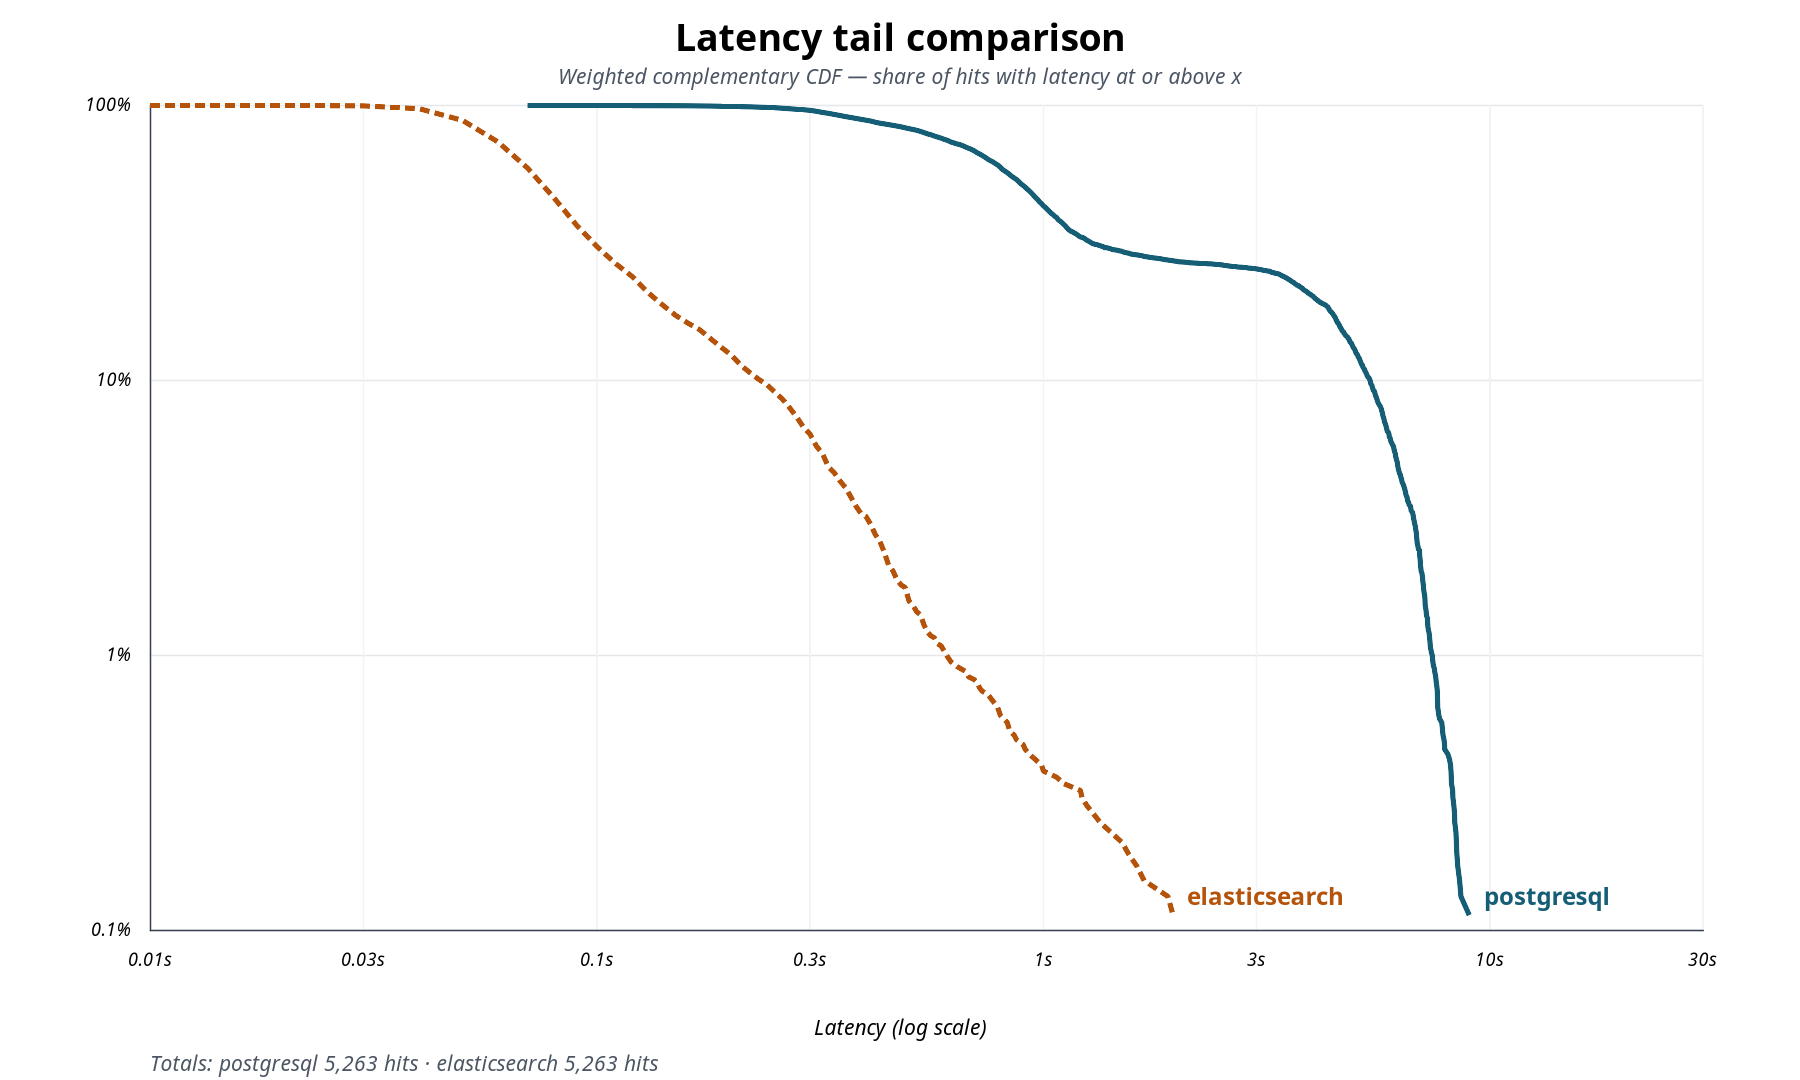
\includegraphics[height=0.74\textheight]{assets/latency-tail-ccdf.png}
\end{frame}

\begin{frame}{Outcome: Reading The Tail}
  \begin{itemize}
    \item Horizontal axis: query latency; lower is faster.
    \item Vertical axis: share of requests at or above that latency.
    \item At 1\%, read the approximate p99 latency.
    \item The Elasticsearch curve is faster, but still has requests above 1 second.
  \end{itemize}
  \begin{block}{Scope}
    The plotted comparison contains 5,263 observations per system. It does not establish a 100 ms maximum or the achieved throughput.
  \end{block}
\end{frame}

\begin{frame}{Outcome: Lessons}
  \begin{itemize}
    \item Search migration is not only a database replacement.
    \item Monitor replication lag and failures; support replay.
    \item Analyzer design matters as much as the search engine.
    \item Ranking metrics are useful, but human judgement can change the decision.
    \item Idempotent writes and checkpoints reduce operational risk.
  \end{itemize}
\end{frame}

\begin{frame}{Outcome: Closing}
  \begin{center}
    \Large
    PostgreSQL remains the source of truth.\\[0.35cm]
    Elasticsearch serves company search.\\[0.35cm]
    \normalsize
    The migration changed ranking and added a replayable indexing pipeline.
  \end{center}
\end{frame}

\begin{frame}[plain]
  \begin{center}
    {\Huge\bfseries\textcolor{PrimaryBlue}{Thank you}}\\[0.7cm]
    {\Large Amir Hossein Rassafi}\\[0.2cm]
    Head of Platform at Condukt\\[0.4cm]
    \href{https://amir-h-rassafi.github.io}{amir-h-rassafi.github.io}
  \end{center}
\end{frame}

\end{document}
